\chapter{Design}

\section{Component diagram}

The system will be organized in a classical client-server configuration, and the latter will expose RESTful APIs to the clients, and a web application for both OPs and PRs. Every service will be in its own servlet. The component diagram is shown in Figure \ref{fig:component}.

\begin{figure}[h]
    \centering
    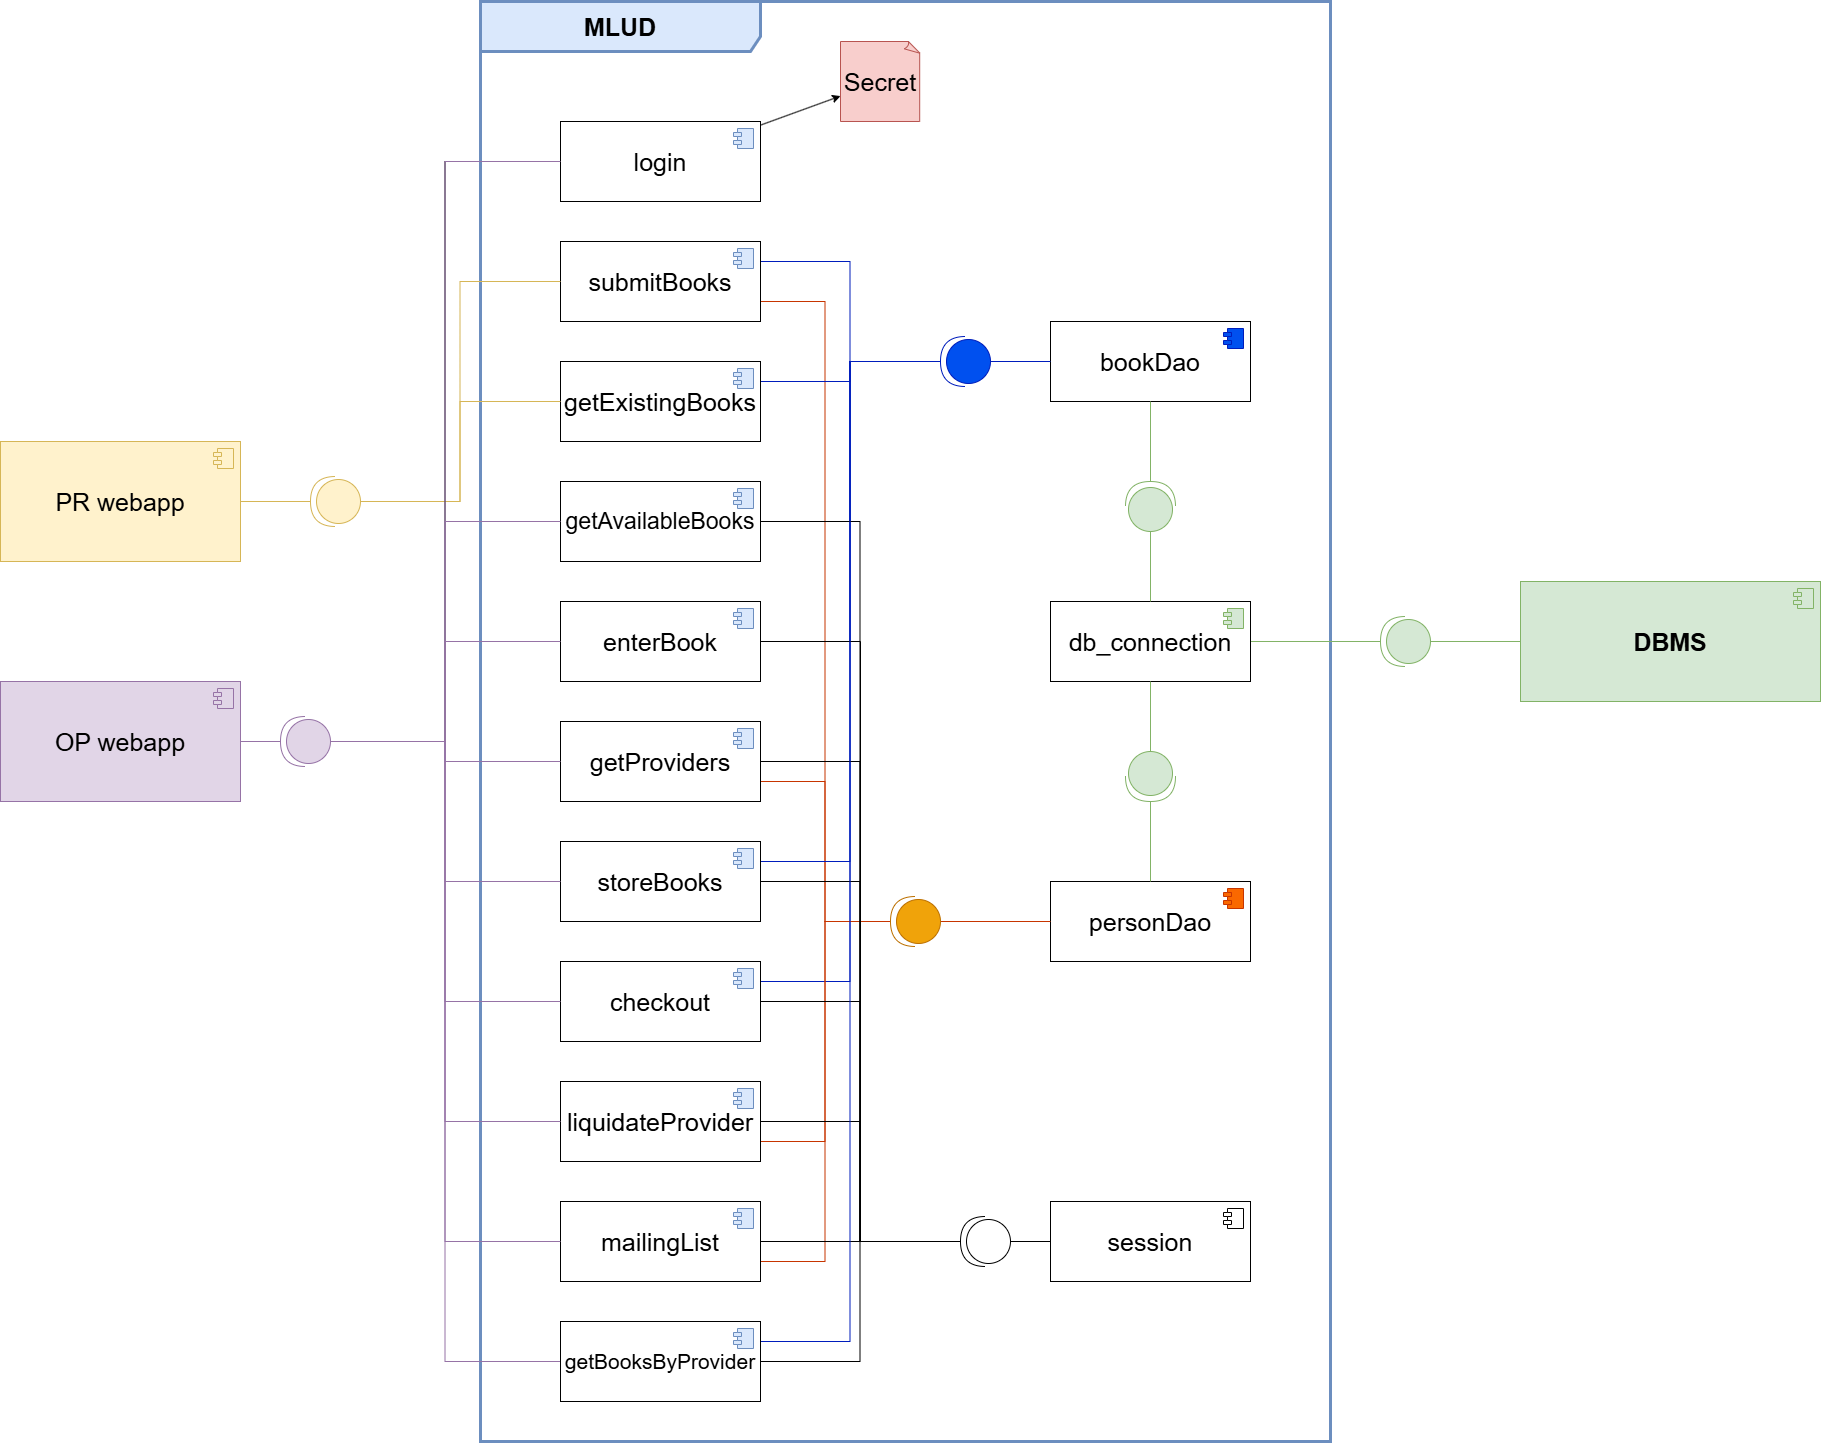
\includegraphics[width=\textwidth]{assets/component_diagram.png}
    \caption{Component diagram}
    \label{fig:component}
\end{figure}

\section{Logical description of data}

The data will be stored into a relational database, which will be designed according to the Logical schema in Figure \ref{fig:er}.

\begin{figure}[h]
    \centering
    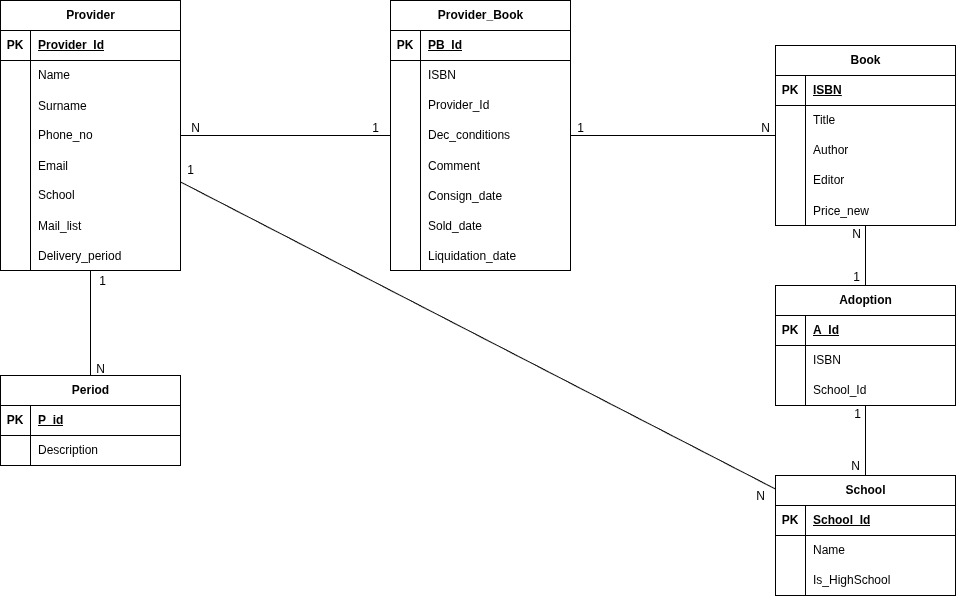
\includegraphics[width=\textwidth]{assets/er_diagram.png}
    \caption{Logical schema of the database}
    \label{fig:er}
\end{figure}

\section{API endpoints}

The API will expose the endpoints in a structure coherent with the compoenent diagram \ref{fig:component}. It follows a list of the endpoints:

\subsection{Login}
\textbf{Method} : POST \\
\textbf{EndPoint} : /login.php \\
\textbf{Body parameters} :
\begin{lstlisting}[language=JavaScript, label={lst:jscode}, basicstyle=\ttfamily]
{ "Password": String }
\end{lstlisting}
\textbf{Response} : \texttt{200} if the login is successful, \texttt{401} if the password is wrong.

\subsection{Submit Books}
A PR submits its books to the system, and gives its personal information.\\
\textbf{Method} : POST \\
\textbf{EndPoint} : /submitBooks.php \\
\textbf{Body parameters} :
\begin{lstlisting}[language=JavaScript, label={lst:jscode}, basicstyle=\ttfamily]
{
    "personalInfo": {
        "Name": String,
        "Surname": String,
        "School": String,
        "Email": String,
        "Phone_no": String,
        "Mail_list": Boolean
    },
    "books": [
        {
            "ISBN": String,
            "Title": String,
            "Author": String,
            "Editor": String,
            "Price_new": Number,
            "Dec_conditions": String
        },
        ...
    ]
}
\end{lstlisting}
\textbf{Response} : \texttt{200} if the submission is successful, \texttt{400} if the request is malformed.

\subsection{Get Existing Books}
The system returns the information of the books already in the system, searching by ISBN or Title, depending on the parameters.\\
\textbf{Method} : GET \\
\textbf{EndPoint} : /getExistingBooks.php \\
\textbf{URL parameters} :
\begin{itemize}
    \item \texttt{ISBN}: String
    \item \texttt{Title}: String
\end{itemize}
\textbf{Response} :
\begin{lstlisting}[language=JavaScript, label={lst:jscode}, basicstyle=\ttfamily]
[
    {
        "ISBN": String,
        "Title": String,
        "Author": String,
        "Editor": String,
        "Price_new": Number
    },
    ...
]
\end{lstlisting}

\subsection{Get Books in Stock}
The system returns all the books in stock, i.e. the books both submitted and actually delivered by the PRs.\\
\textbf{Method} : GET \\
\textbf{EndPoint} : /getAvailableBooks.php \\
\textbf{Response} :
\begin{lstlisting}[language=JavaScript, label={lst:jscode}, basicstyle=\ttfamily]
[
    {
        "ISBN": String,
        "Title": String,
        "Author": String,
        "Editor": String,
        "Price_new": Number,
        "ProviderName": String,
        "ProviderSurname": String,
        "PB_Id": Number,
        "Provider_Id": Number,
        "Dec_conditions": String,
        "Comment"? : String,
        "Consign_date": String,
        "Sold_date": null, 
        "Liquidation_date": null

    },
    ...
]
\end{lstlisting}

\subsection{Enter book}
An OP enters a book in the system, associating it to a ISBN. No strong need for this, it's just to make simpler the PR submission.\\
\textbf{Method} : POST \\
\textbf{EndPoint} : /enterBook.php \\
\textbf{Body parameters} :
\begin{lstlisting}[language=JavaScript, label={lst:jscode}, basicstyle=\ttfamily]
{
    "ISBN": String,
    "Title": String,
    "Author": String,
    "Editor": String,
    "Price_new": Number
}
\end{lstlisting}
\textbf{Response} : \texttt{200} if the submission is successful, \texttt{400} if the request is malformed.

\subsection{Get PRs}
The system returns the list of PRs.
\textbf{Method} : GET \\
\textbf{EndPoint} : /getProviders.php \\
\textbf{Response} :
\begin{lstlisting}[language=JavaScript, label={lst:jscode}, basicstyle=\ttfamily]
[
    {
        "Provider_Id": Number,
        "Name": String,
        "Surname": String,
        "State": String
    },
    ...
]
\end{lstlisting}
The possible states are:
\begin{itemize}
    \item \texttt{0} - waiting for delivery
    \item \texttt{1} - waiting for liquidation
    \item \texttt{2} - liquidated
\end{itemize}

\subsection{Get Books submitted by a PR}
The system returns the books submitted by a PR. Useful for book delivery\\
\textbf{Method} : GET \\
\textbf{EndPoint} : /getBooksByProvider.php \\
\textbf{URL parameters} :
\begin{itemize}
    \item \texttt{Provider\_Id}: Number
\end{itemize}
\textbf{Response} :
\begin{lstlisting}[language=JavaScript, label={lst:jscode}, basicstyle=\ttfamily]
{
    "books": [
        {
            "PB_Id": Number,
            "ISBN": String,
            "Title": String,
            "Author": String,
            "Editor": String,
            "Price_new": Number,
            "Dec_conditions": String,
            "Sold_date": Timestamp
        },
        ...
    ],
    "provider": [
        {
            "Name": String,
            "Surname": String
        }
    ]
}
\end{lstlisting}

\subsection{Deliver Books}
A PR delivers the books to the OP.\\
\textbf{Method} : POST \\
\textbf{EndPoint} : /storeBooks.php \\
\textbf{Body parameters} :
\begin{lstlisting}[language=JavaScript, label={lst:jscode}, basicstyle=\ttfamily]
{
    "Provider_Id": Number,
    "Books_to_edit": [
        {
            "PB_Id": Number,
            "Dec_conditions": String,
            "Comment"?: String
        },
        ...
    ],
    "Books_to_add": [
        {
            "ISBN": String,
            "Title": String,
            "Author": String,
            "Editor": String,
            "Price_new": Number,
            "Dec_conditions": String,
            "Comment"?: String
        },
        ...
    ],
    "Books_to_remove": [
        { "PB_Id": Number },
        ...
    ]
}
\end{lstlisting}
\textbf{Response} : \texttt{200} if the submission is successful, \texttt{400} if the request is malformed.

\subsection{Sell Books}
An OP sells the books to a BY.\\
\textbf{Method} : POST \\
\textbf{EndPoint} : /checkout.php \\
\textbf{Body parameters} :
\begin{lstlisting}[language=JavaScript, label={lst:jscode}, basicstyle=\ttfamily]
[
    { "PB_Id": Number },
    ...
]
\end{lstlisting}
\textbf{Response} : \texttt{200} if the submission is successful, \texttt{400} if the request is malformed.

\subsection{Get Situation for a PR after delivery}
The system returns the situation of a PR after the delivery: unsold books and how much money the PR has to receive.\\
\textbf{Method} : GET \\
\textbf{EndPoint} : /getSituation.php \\
\textbf{URL parameters} :
\begin{itemize}
    \item \texttt{Provider\_Id}: Number
\end{itemize}
\textbf{Response} :
\begin{lstlisting}[language=JavaScript, label={lst:jscode}, basicstyle=\ttfamily]
{
    "Name": String,
    "Surname": String,
    "Unsold_books": [
        {
            "PB_Id": Number,
            "ISBN": String,
            "Title": String,
            "Author": String,
            "Editor": String,
            "Price_new": Number,
            "Dec_conditions": String
        },
        ...
    ],
    "Money": Number
}
\end{lstlisting}

\subsection{Liquidate PR and return unsold books}
An OP liquidates the PR, returning the unsold books and the money.\\
\textbf{Method} : POST \\
\textbf{EndPoint} : /liquidateProvider.php \\
\textbf{Body parameters} :
\begin{lstlisting}[language=JavaScript, label={lst:jscode}, basicstyle=\ttfamily]
{ "Provider_Id": Number, }
\end{lstlisting}
\textbf{Response} : \texttt{200} if the submission is successful, \texttt{400} if the request is malformed.

\subsection{Mailing list}
Show the list of PRs that accepted to be in the mailing list.\\
\textbf{Method} : GET \\
\textbf{EndPoint} : /mailingList.php \\
\textbf{Response} :
\begin{lstlisting}[language=JavaScript, label={lst:jscode}, basicstyle=\ttfamily]
[
    {
        "Name": String,
        "Surname": String,
        "Phone_no": String,
        "Email": String,
        "School": String,
        "Mail_list": Boolean
    },
    ...
]
\end{lstlisting}

\subsection{Session check}
Check if the session is still valid.\\
\textbf{Method} : GET \\
\textbf{EndPoint} : /utils/session.php \\
\textbf{Response} : \texttt{200} if the session is still valid, \texttt{401} if the session is expired.

\subsection{Logout}
Logout the OP.\\
\textbf{Method} : GET \\
\textbf{EndPoint} : /logout.php \\
\textbf{Response} : \texttt{200} if the logout is successful.

\subsection{Get Schools}
When a PR starts to fill the form, it has to select its school of origin. The system returns the list of schools.\\
\textbf{Method} : GET \\
\textbf{EndPoint} : /getSchools.php \\
\textbf{Response} :
\begin{lstlisting}[language=JavaScript, label={lst:jscode}, basicstyle=\ttfamily]
[
    {
        "School_Id": Number,
        "Name": String,
        "Is_HighSchool": Boolean
    },
    ...
]
\end{lstlisting}

\subsection{Get Book Adopted by a School}
When a PR fills the "school of origin" field, the system suggests the books adopted by that school.\\
\textbf{Method} : GET \\
\textbf{EndPoint} : /getAdoptedBooks.php \\
\textbf{URL parameters} :
\begin{itemize}
    \item \texttt{School\_Id}: Number
\end{itemize}
\textbf{Response} :
\begin{lstlisting}[language=JavaScript, label={lst:jscode}, basicstyle=\ttfamily]
[
    {
        "ISBN": String,
        "Title": String,
        "Author": String,
        "Editor": String,
        "Price_new": Number
    },
    ...
]
\end{lstlisting}

\subsection{Get periods of delivery and number of PRs}
When a PR fills the "period of delivery" field, the system suggests the periods of delivery and the number of PRs that have already submitted the form for that period.\\
\textbf{Method} : GET \\
\textbf{EndPoint} : /getPeriodsAndAffluences.php \\
\textbf{Response} :
\begin{lstlisting}[language=JavaScript, label={lst:jscode}, basicstyle=\ttfamily]
[
    {
        "P_Id": Number,
        "Description": String,
        "Num_Providers": Number
    },
    ...
]
\end{lstlisting}

\subsection{Get Emails subscribed grouped by period}
When an OP wants to send an email to the PRs, it can select a period and the system returns the emails of the PRs that subscribed to the mailing list for that period.\\
\textbf{Method} : GET \\
\textbf{EndPoint} : /getPersonsByPeriod.php \\
\textbf{Response} :
\begin{lstlisting}[language=JavaScript, label={lst:jscode}, basicstyle=\ttfamily]
[
    {
        "period_Description": String,
        "emails": [
            String,
            ...
        ]
    },
    ...
]
\end{lstlisting}

\section{Deployment}

All the webapp will be entirely deployed on the free hosting service \href{www.altervista.org}{Altervista}, which provides a MySQL database and a php server, so all the problems of deployment, reliability, scalability, and security are handled by the service provider.

Particularly, the link to the webapp will be \url{https://lokalinomlud.altervista.org/}

\section{UX design}

The webapp will be designed with a simple and intuitive interface, with a clean and modern look.

The UX is explained at an high level in the flow diagrams in Figures \ref{fig:flow_book_submission} and \ref{fig:flow_op}.

\begin{figure}[ht]
    \centering
    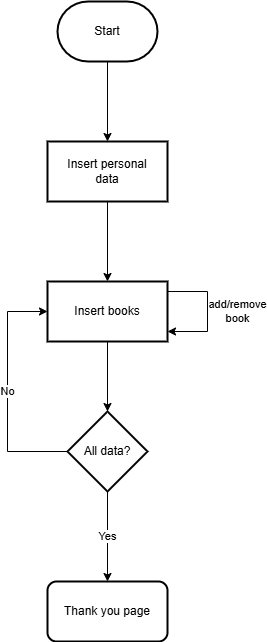
\includegraphics[width=.25\textwidth]{assets/flow_book_submission.png}
    \caption{Flow of the book submission}
    \label{fig:flow_book_submission}
\end{figure}

\begin{figure}[ht]
    \centering
    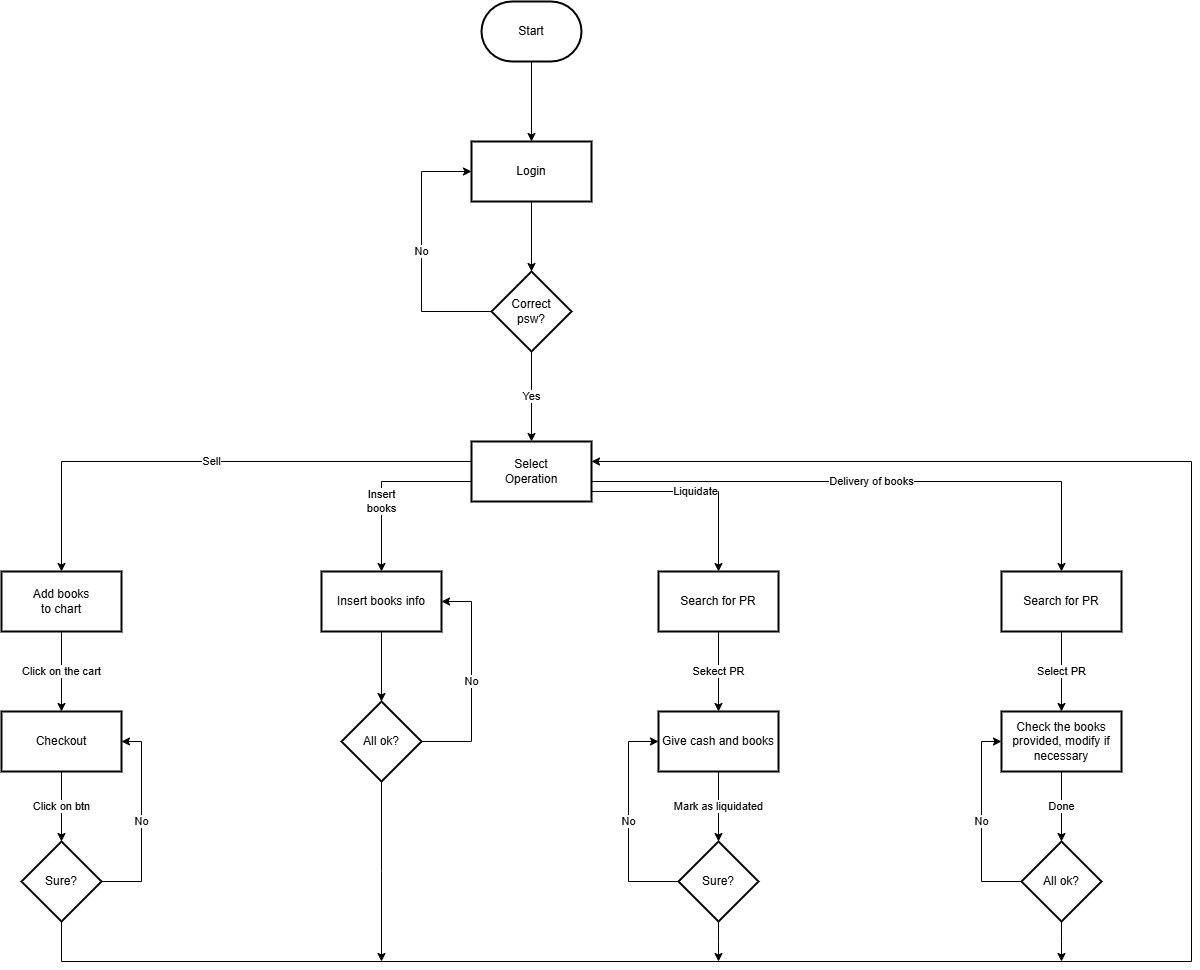
\includegraphics[width=\textwidth]{assets/flow_op.png}
    \caption{Flow of the OP}
    \label{fig:flow_op}
\end{figure}

\section{User interface}
\label{sec:ui}

\begin{figure}[ht]
    \centering
    
\includegraphics[width=.5\textwidth]{assets/ui_mockup/login.png}
    \caption{Login page}
    \label{fig:login}
\end{figure}

\begin{figure}[ht]
    \centering
    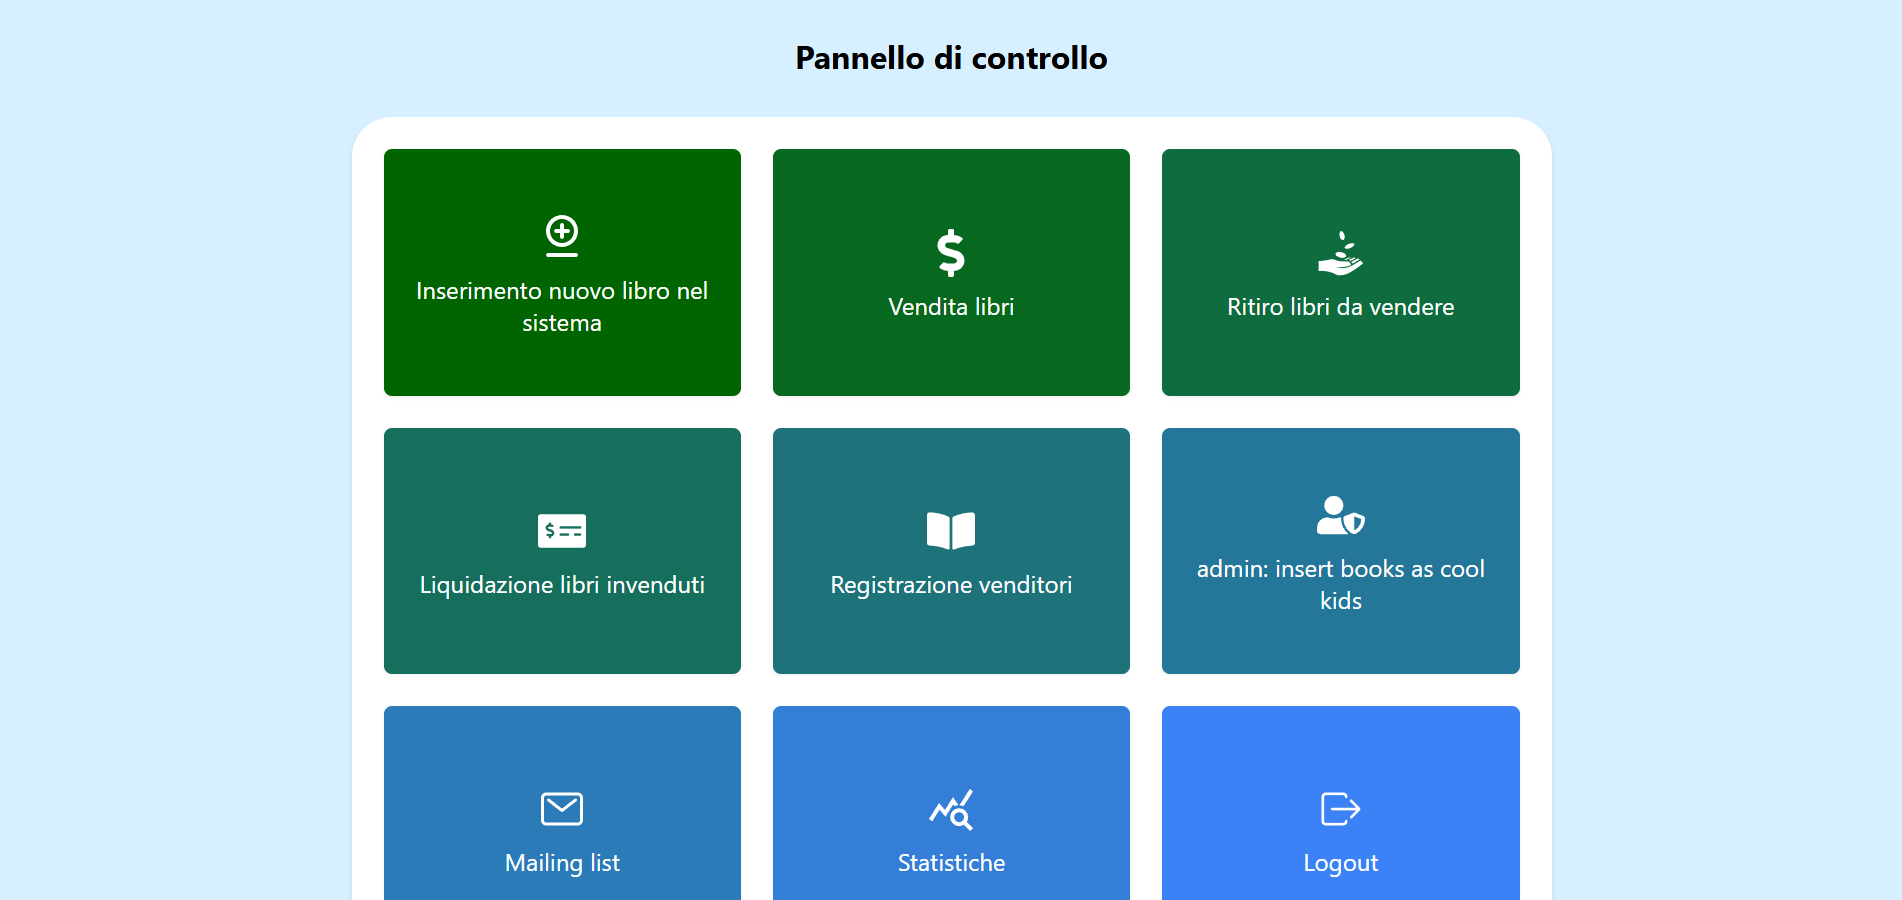
\includegraphics[width=.75\textwidth]{assets/ui_mockup/dashboard.png}
    \caption{Dashboard}
    \label{fig:dashboard}
\end{figure}

\begin{figure}[ht]
    \centering
    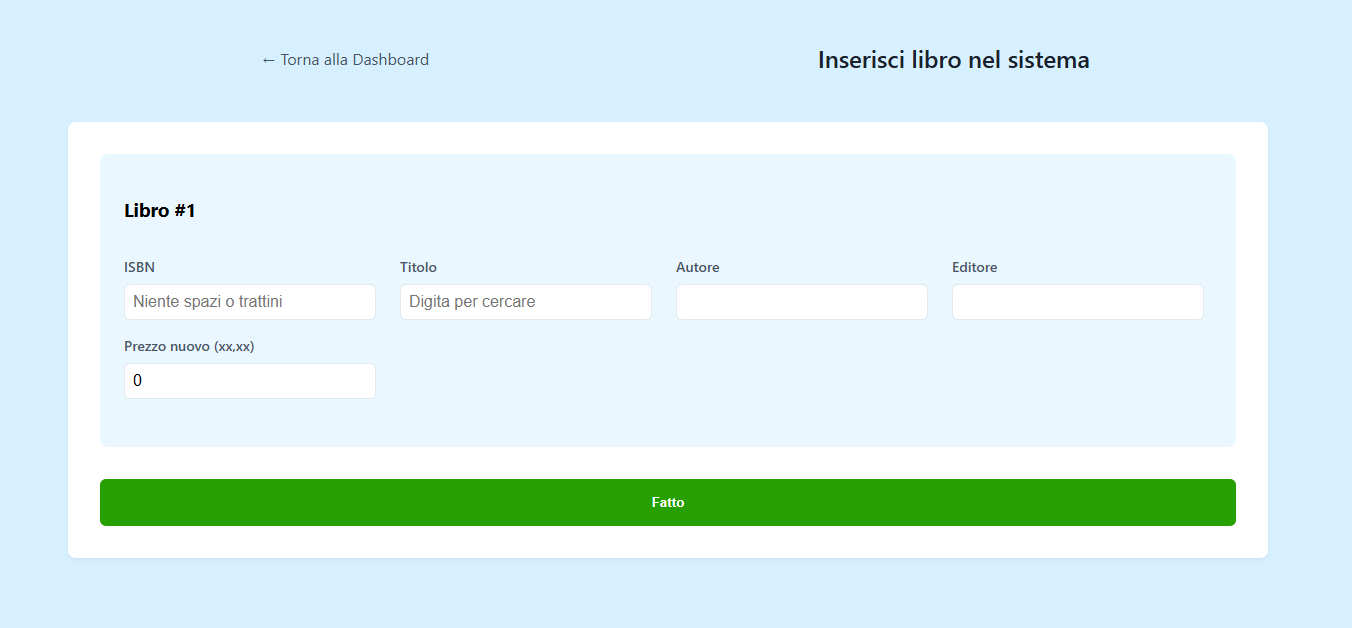
\includegraphics[width=.75\textwidth]{assets/ui_mockup/insert_book.png}
    \caption{Insert book into the system}
    \label{fig:insert_book}
\end{figure}

\begin{figure}[ht]
    \centering
    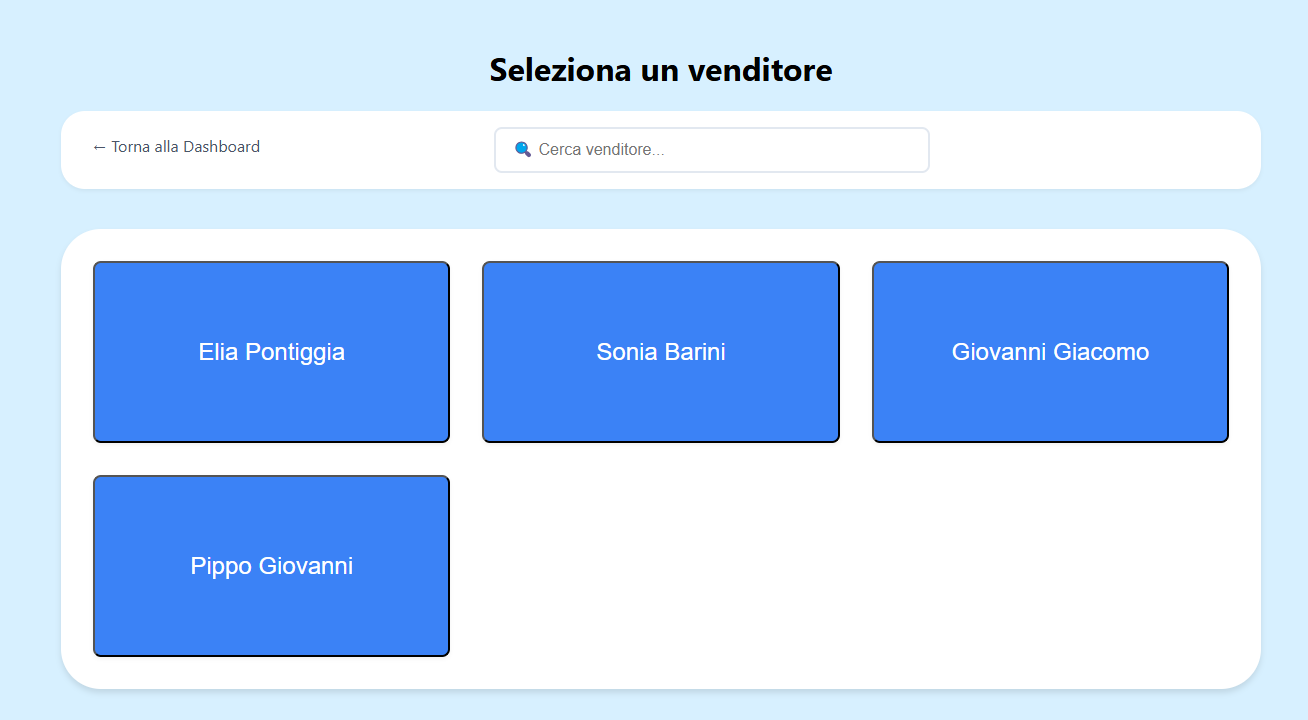
\includegraphics[width=.75\textwidth]{assets/ui_mockup/pickup_pr.png}
    \caption{Select a PR to pick up its books}
    \label{fig:pickup_pr}
\end{figure}

\begin{figure}[ht]
    \centering
    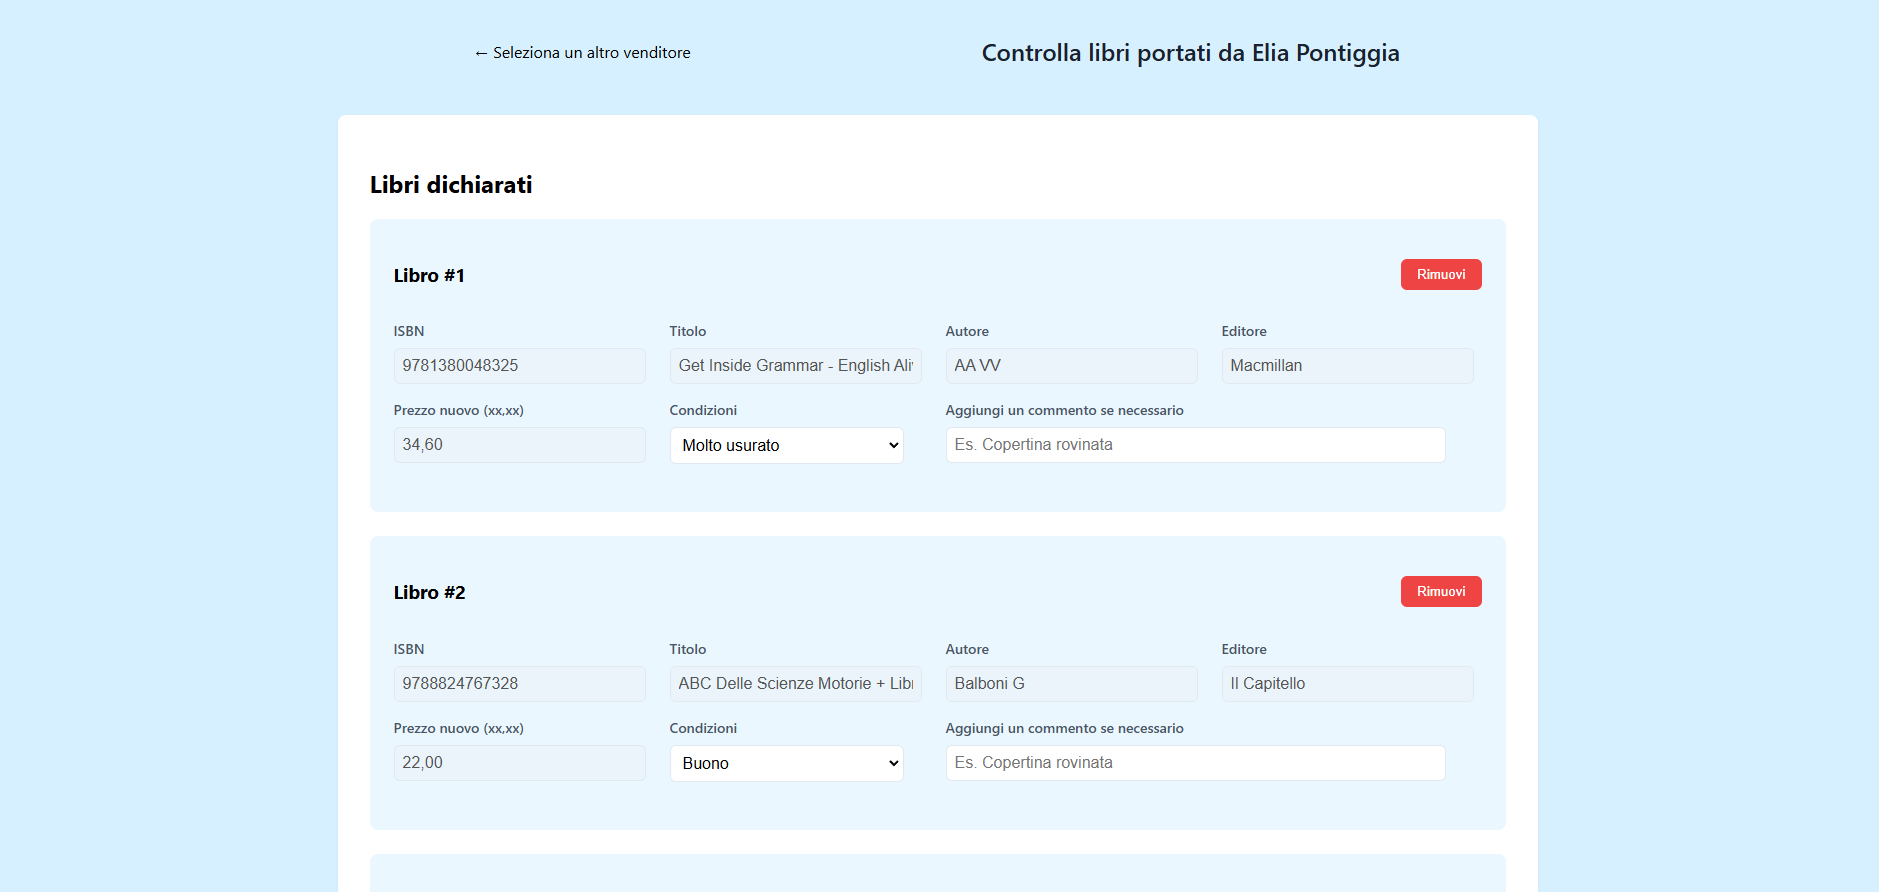
\includegraphics[width=.75\textwidth]{assets/ui_mockup/pickup_list.png}
    \caption{List of books to pick up from a PR}
    \label{fig:pickup_list}
\end{figure}

\begin{figure}[ht]
    \centering
    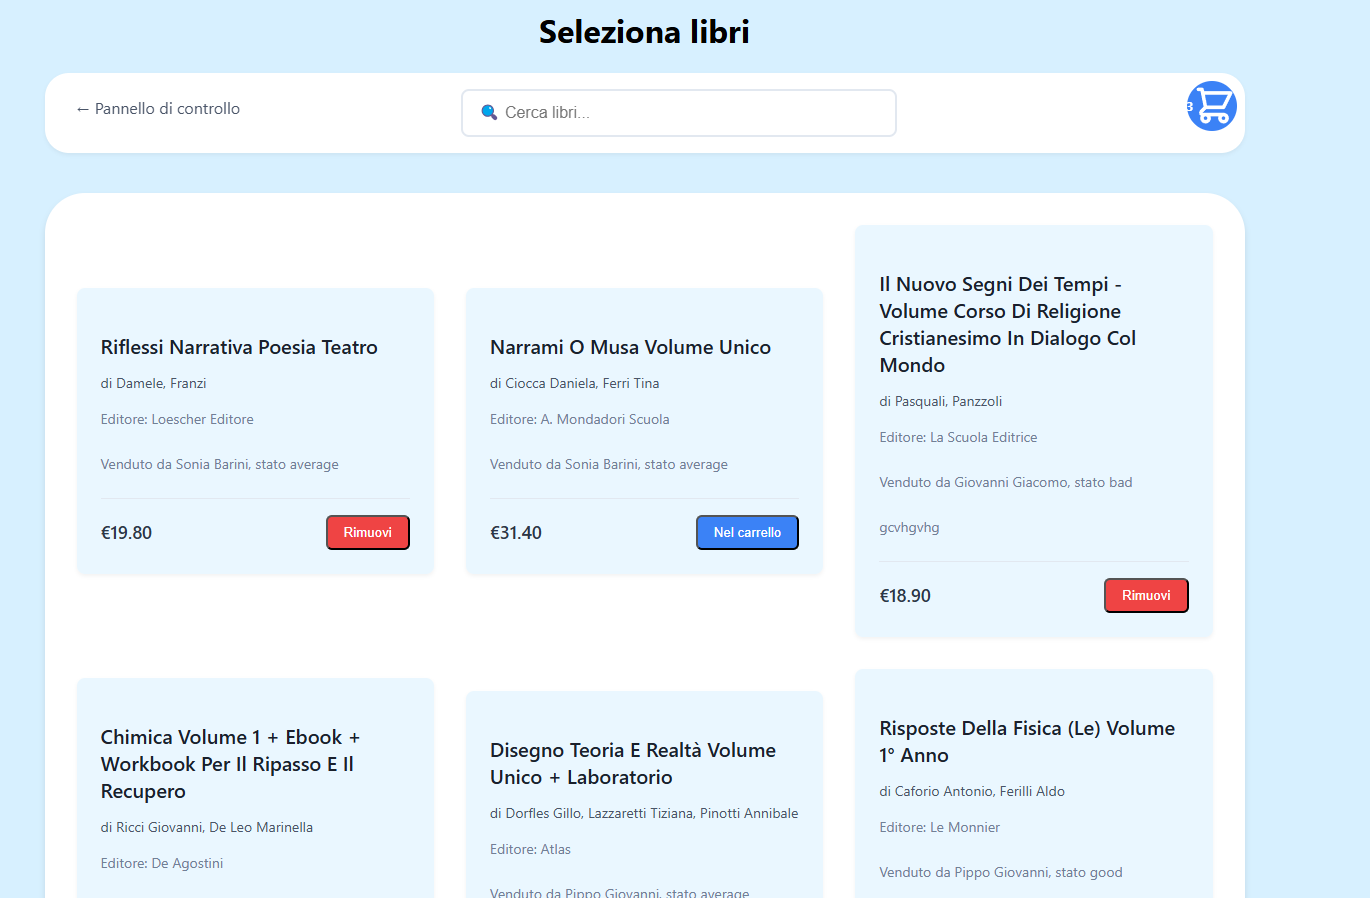
\includegraphics[width=.75\textwidth]{assets/ui_mockup/sellpage.png}
    \caption{Books to sell}
    \label{fig:sellpage}
\end{figure}

\begin{figure}[ht]
    \centering
    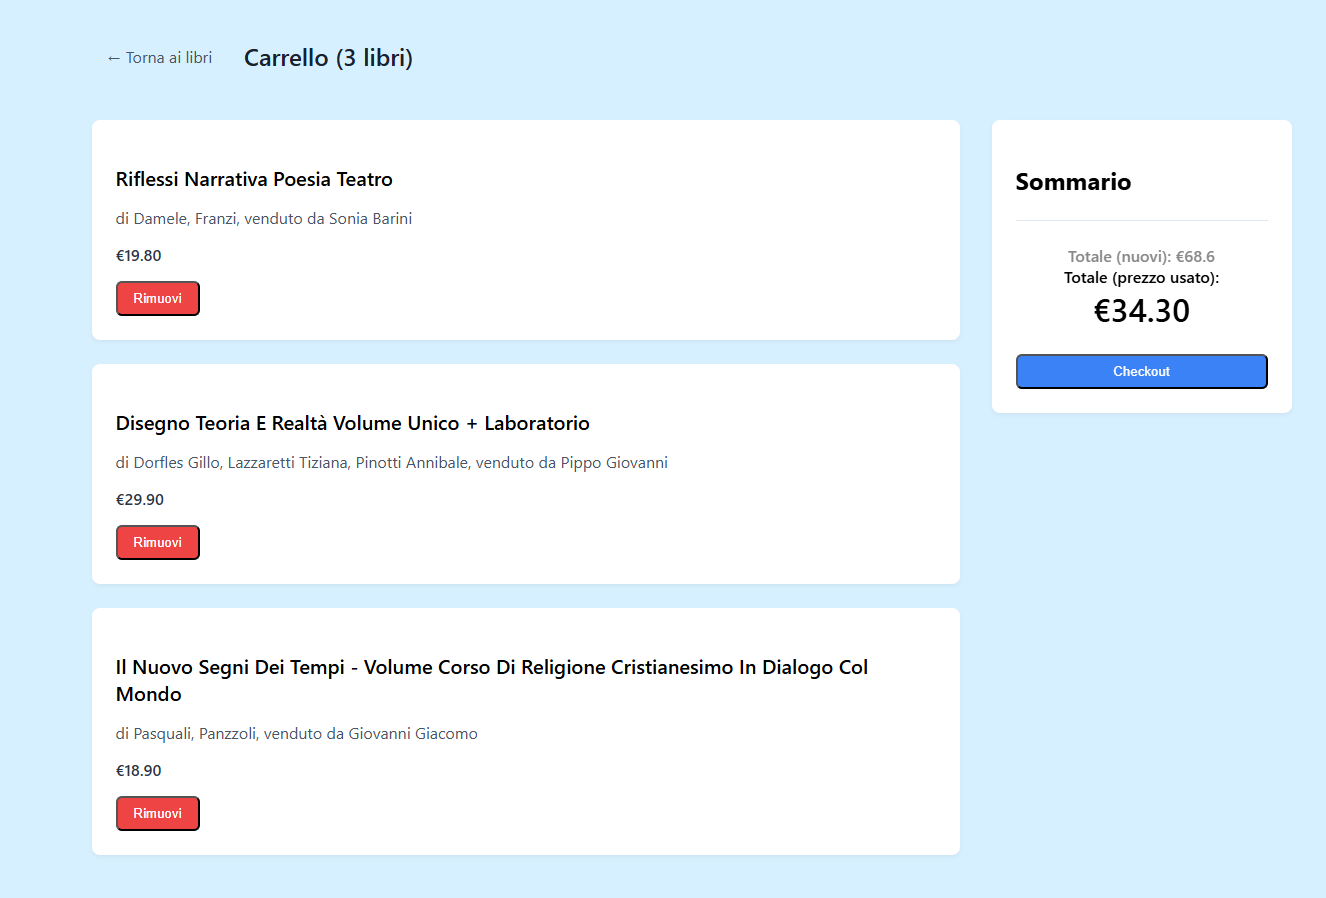
\includegraphics[width=.75\textwidth]{assets/ui_mockup/cart.png}
    \caption{Cart}
    \label{fig:cart}
\end{figure}

\begin{figure}[ht]
    \centering
    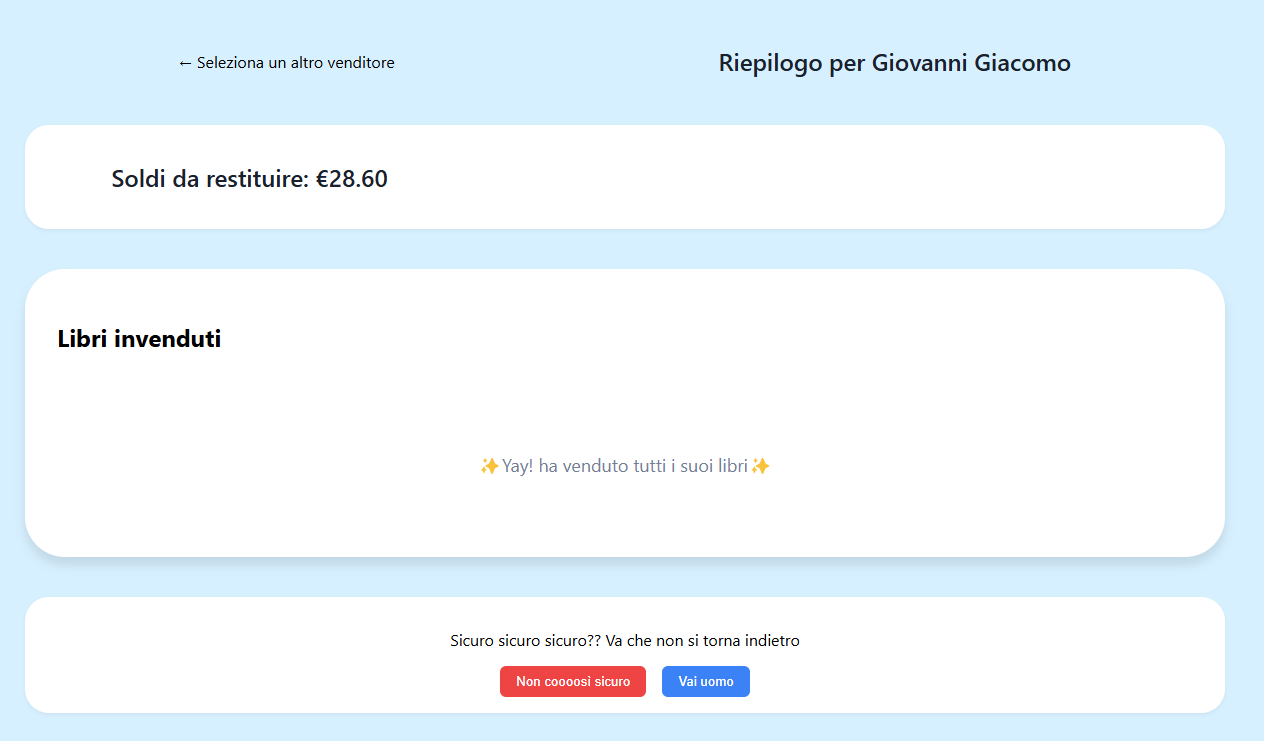
\includegraphics[width=.75\textwidth]{assets/ui_mockup/liquidation.png}
    \caption{Liquidation of a PR}
    \label{fig:liquidation}
\end{figure}

\begin{figure}[ht]
    \centering
    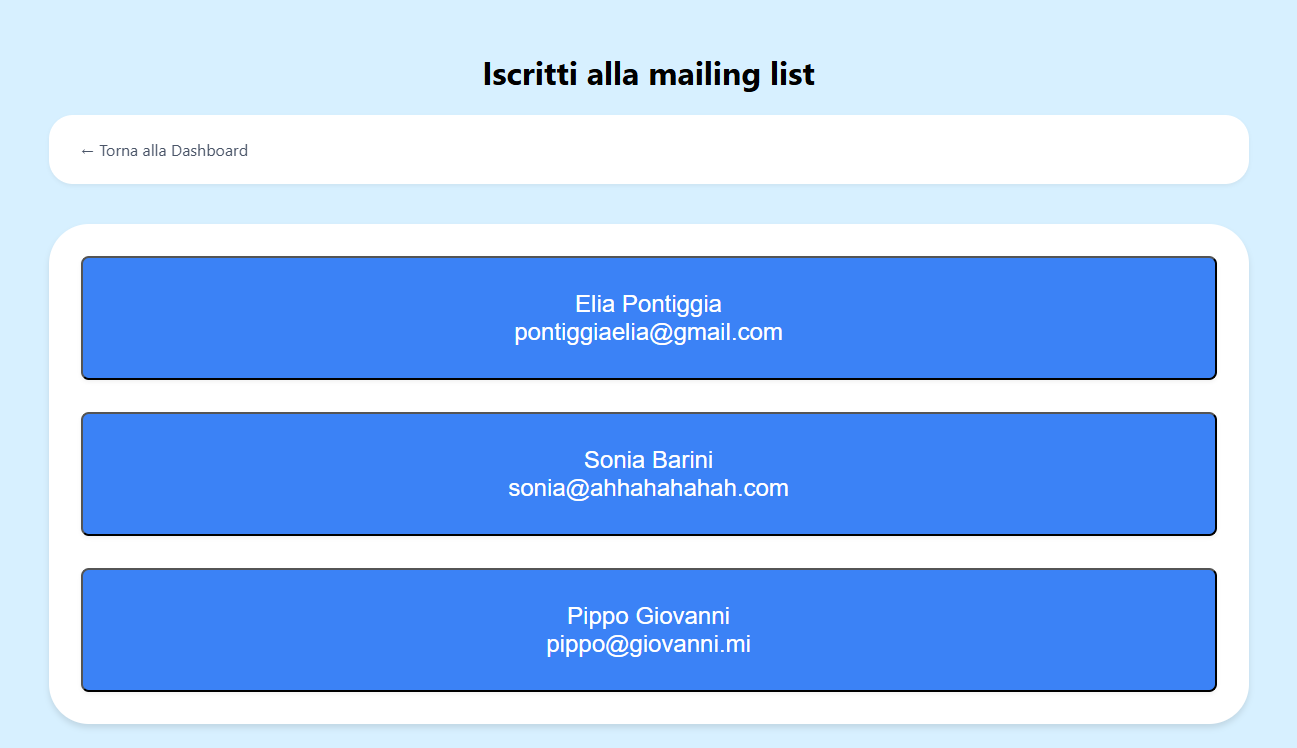
\includegraphics[width=.75\textwidth]{assets/ui_mockup/mailinglist.png}
    \caption{Mailing list}
    \label{fig:mailinglist}
\end{figure}

\begin{figure}[ht]
    \centering
    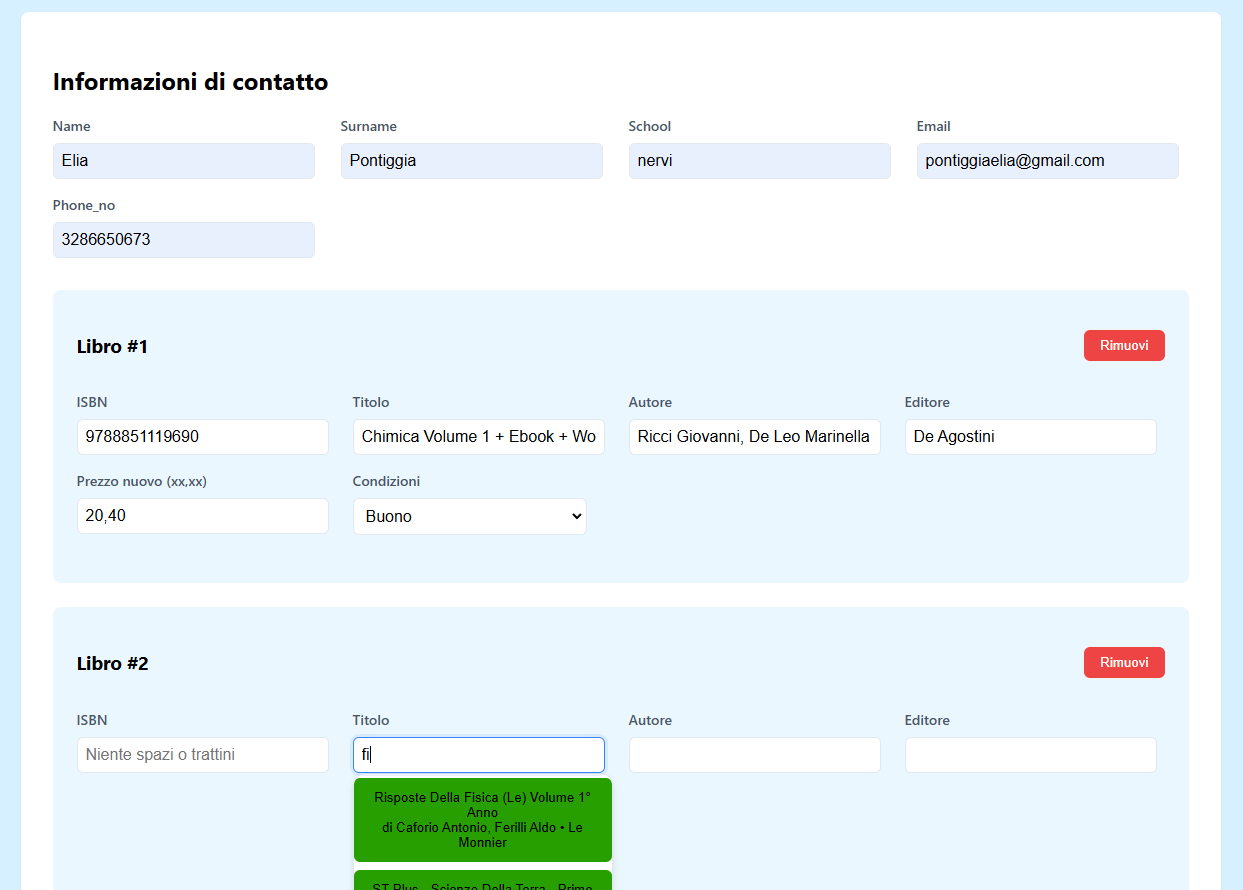
\includegraphics[width=.65\textwidth]{assets/ui_mockup/booksubmissionform.png}
    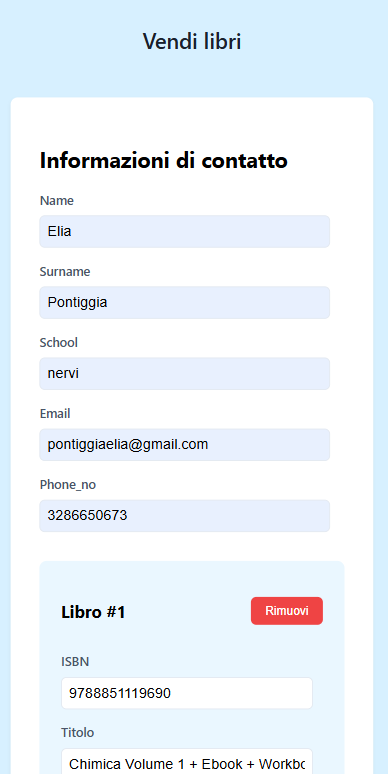
\includegraphics[width=.30\textwidth]{assets/ui_mockup/booksubmissionsmartphone.png}
    \caption{PR registration in both scenarios: from a PC and from a smartphone}
    \label{fig:booksubmissionform}
\end{figure}